\section{Introduction}
\label{sec:intro}

Online user review is an integral part of e-commerce. Popular e-commerce
websites feature enormous amount of text reviews, especially for popular
products and services. To improve the user experience and expedite the
shopping process, many websites provides either qualitative or quantitative
summary of the user reviews, organized by important aspects or characteristics
of the target product or service.
Two examples of such \emph{aspect-based review 
summarization}~\cite{hu2004mining} are shown in \figref{fig:tripadvisor} 
and \figref{fig:cars.com}. In \figref{fig:tripadvisor} from TripAdvisor, 
besides the short review passage written by the user, the user are asked
to give discrete ratings (on the scale of 1-5) on various aspects of 
the hotel room, e.g., location and cleanness. The ratings of 
a product from individual reviews can then be aggregated into an overall
ratings of the same product by many users, such as those shown
about a specific car model in \figref{fig:cars.com}, a snapshot from Cars.com. 
%Aspect-based review summarization is commonly seen on websites 
%like TripAdvisor and Cars.com. 

Aspect-based reviews have several advantages compared to the more traditional 
style of online reviews that consists of a short passage and an overall rating. 
In aspect-based reviews, more details are provided quantitatively and 
more directly, and the users can learn about various aspects of a product 
without having to read the entire review passage. Another advantage of 
aspect-based reviews is that different products within the same category 
can be compared directly with respect to multiple aspects, 
instead of just an overall rating. When researching on products, 
users spend most of their time comparing different brands and models. 
Aspect-based review summarization provides an effective and efficient way for 
doing such comparison, saving the users both time and effort.


\begin{figure}[th]
\centering
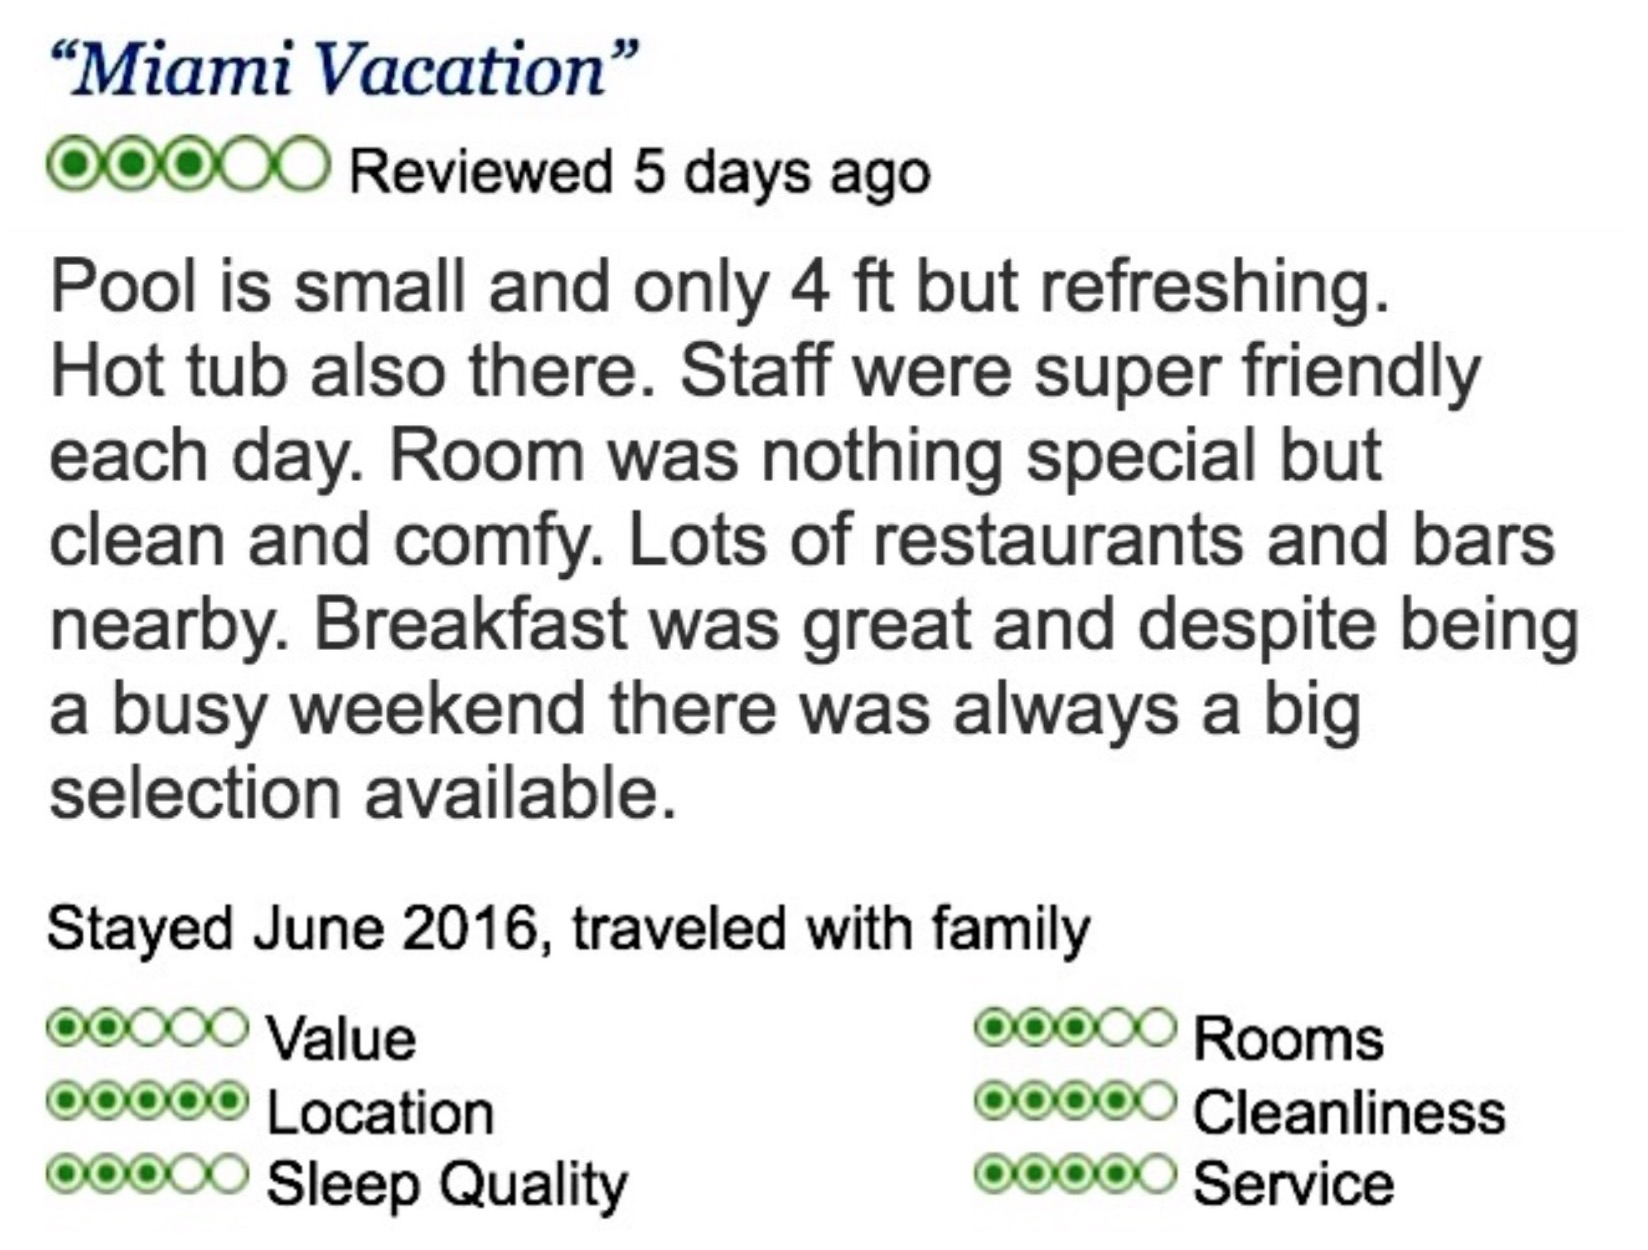
\includegraphics[width=0.7\columnwidth]{figures/tripadvisor}
\caption{User review from TripAdvisor.}
\label{fig:tripadvisor}
\end{figure}

\begin{figure}[th]
\centering
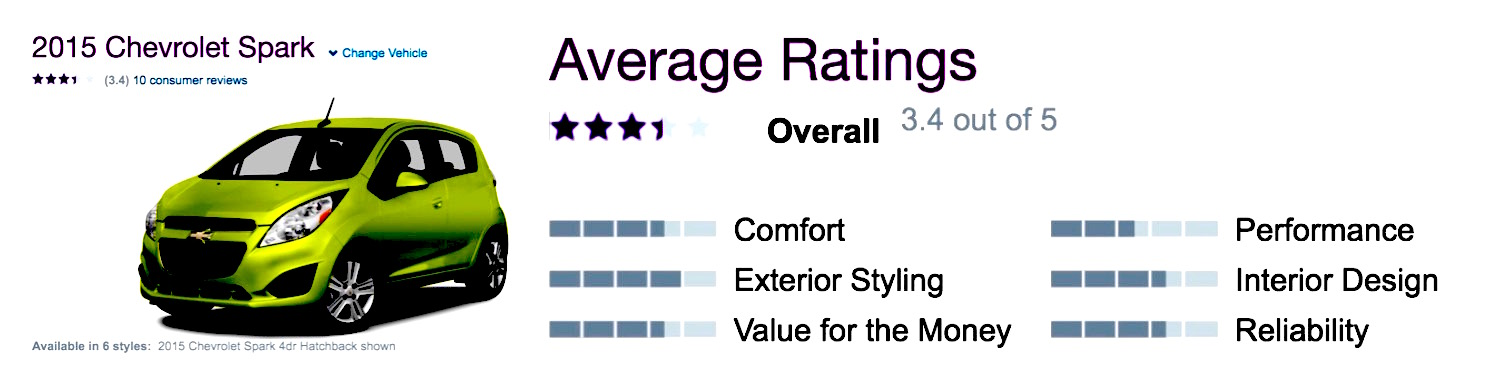
\includegraphics[width=1.0\columnwidth]{figures/cars}
\caption{Review summarization from Cars.com.}
\label{fig:cars.com}
\end{figure}

At present, websites that offer aspect-based review summaries typically 
only feature a single or a small number of product categories, e.g.,
TripAdvisor.com only features travel related products while Cars.com reviews
automobiles. The reason is that it takes in-depth knowledge to be able to
best characterize a product type using a few keywords, that are both
relevant to the current user interests and diverse enough to cover as many
facets of the type as possible. It is such a difficult task
that these aspects are mostly manually chosen by the website operators.
Manual selection of aspects certainly cannot scale to large number of
product types as featured by general e-commerce platforms such as Amazon,
Taobao and Yelp. These platforms instead turn to automatic review 
summarization, mined from the user review texts. 

\begin{figure}[th]
\centering
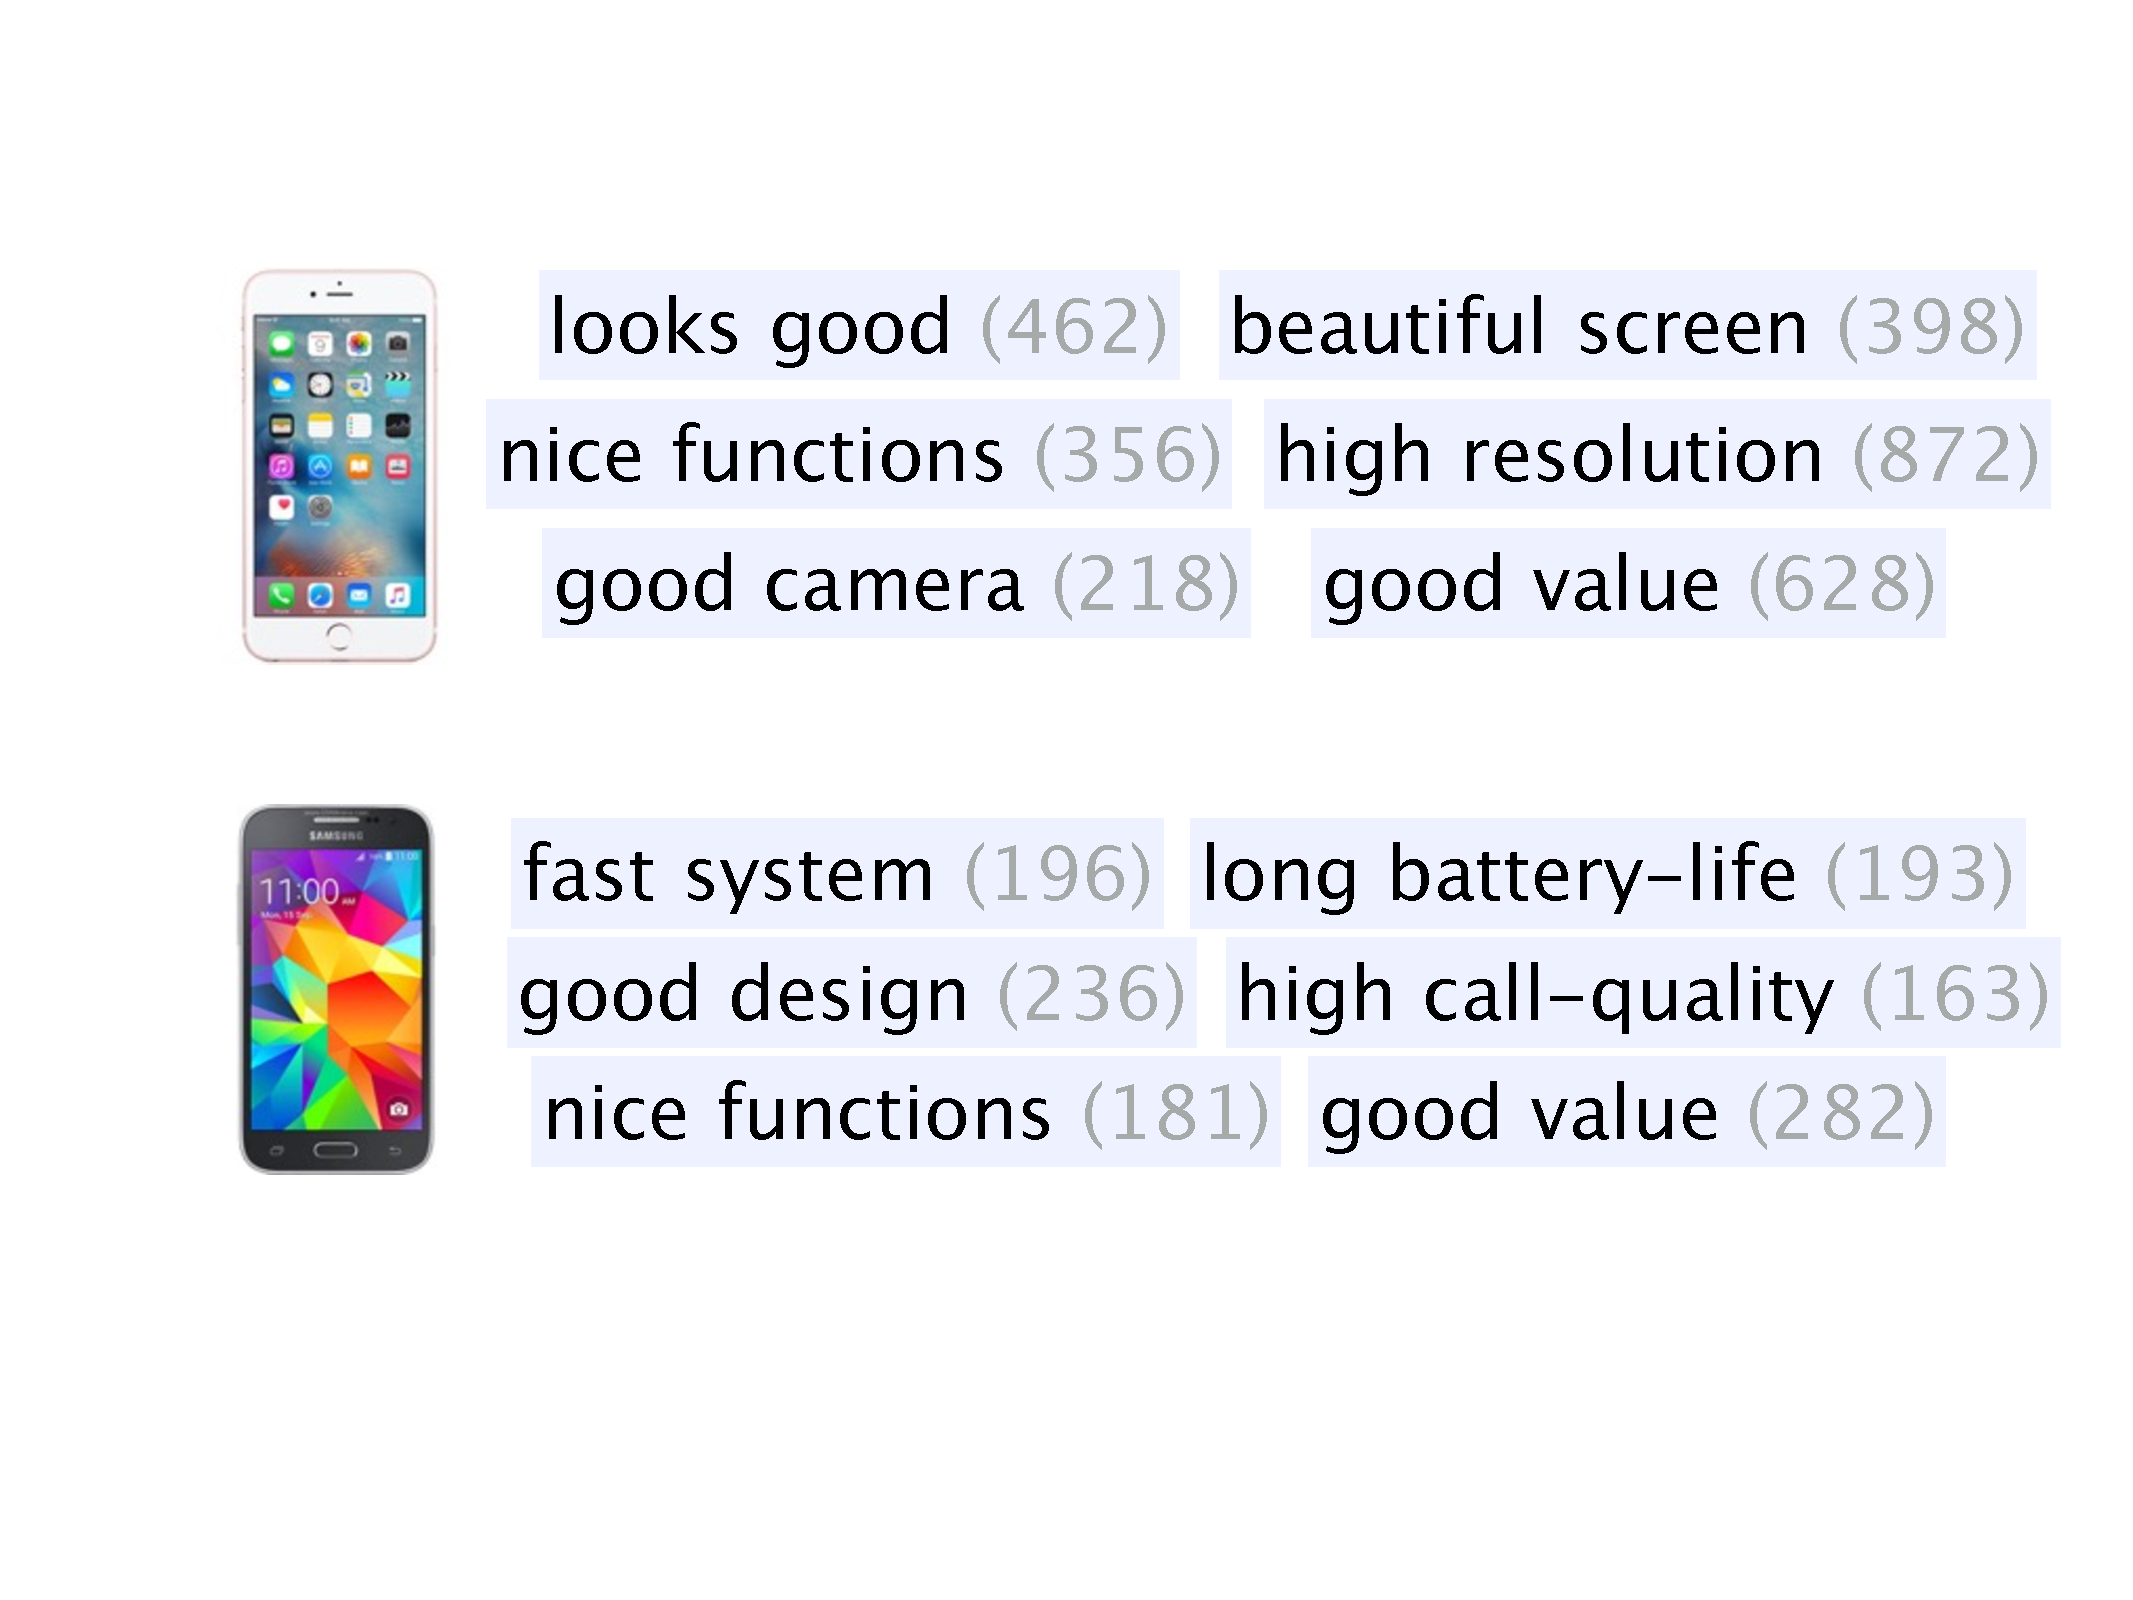
\includegraphics[width=0.8\columnwidth]{figures/phrases}
\caption{Automatic review summarization for two mobile phones 
on an e-commerce website}
\label{fig:phrases}
\end{figure}

An example of automatic review summarization commonly seen 
on e-commerce websites is shown in \figref{fig:phrases}. 
There is a summary of opinion phrases for each phone model, 
along with the frequency of each phrase mentioned in the 
reviews. There are two major drawbacks in this form of summarization. 
First, it is restricted to using the reviews about a specific product. 
Therefore, summaries are incompatible across different products within 
the same category - different models may not share the same set of 
opinion phrases. This makes it less useful for users to compare
different models.  Second, users' sentiment toward 
each aspect cannot be quantified and computationally compared - 
the difference of emotional strength between 
``extremely good" and ``above average" is hard to capture.
% user cannot choose to express them differently.

%The aspects of a product are supposed to capture the most important features 
%and cover all the facets of the product. The products of the same category 
%share the same set of aspects, however the aspects can be very different 
%across categories. It takes both common knowledge and personal experience 
%with the product to decide which are the appropriate aspects. 
%The websites that can provide aspect-based rating system basically 
%all share a common feature, that is they each focuses on only one or 
%a small range of products. For example TripAdvisor focuses on hotels and 
%Cars.com focuese on cars. The set of aspects is what the consumers base 
%on to compare different products, thus they must be carefully chosen 
%to cover all the facest of the product. Moreoever, at the end of the day 
%the aspects is designed to serve the consumers, especially potential consumers, 
%so they need to reflect what the consumers care about the product. 
%Ideally, the aspects should be decided with user reviews taken into 
%consideration. For a small range of products, the website owner or 
%the retailer may manual designate the set of aspects, 
%however this is intractable for websites like Amazon and TaoBao, 
%which host basically all kinds of products available on the market, 
%and websites like Yelp on which users review thousands of different services. 
%
%Motivated by this observation, we are in need for methods that automatically 
%generate review summarizations. 

Our goal in this paper is to develop an unsupervised system 
for aspect word extraction from a set of user reviews about products within 
the same category.  The formulation of aspects extraction, 
which is extracting words from a set of documents, 
is similar to topic modeling where aspects can be seen as topics. 
However, there are three main factors that make aspect extraction 
more challenging:
\begin{itemize}
    \item In topic modeling, there is no restriction on the relationship 
between the topics. In aspect extraction, however, we expect the final 
	aspect words to have small semantic overlap with each other, 
	otherwise the vagueness would confuse the consumers.
    \item The expression of opinions can be very versatile. 
          In user reviews, aspects can appear both explicitly by 
	direct reference, and implicity through users' personal experience.
    \item Opinions about various aspects are expressed within a short 
          piece of text, so the topics may shift very quickly from 
          sentence to sentence.
          Sentences close to each other can often 
          talk about very different topics.
\end{itemize}
Most previously proposed unsupervised methods for aspect extraction are 
variations of topic models. The main problem with topic-model-based methods 
is they leverage only word frequencies and co-occurrances, not word semantics, 
so they cannot effectively leverage the sentences that implicitly discuss 
the product aspects. In our method we leverage the distributed 
representations of words and sentences. With distributed representations, 
the semantic similarity between two sentences can be more accurately 
calculated without relying too much on the lexical information.
Our proposed method consists 3 clustering steps and
2 ranking phase. With a focus on aspect extraction as part of 
review summarization, this paper has two main contributions:

\begin{itemize}
    \item Proposed a new framekwork of unsupervised method for aspect extraction, as an alternative to topic models.
    \item Acheived state-of-the-art performance in end-to-end aspect extraction in multiple domains.
\end{itemize}

In \secref{sec:method} we introduce our method step-by-step.
In \secref{sec:experiments} 
we evaluate our method on user reviews from multiple domains and demonstrate 
the effectiveness of our model against other approaches 
and show how the aspects extracted can be used
to construct a complete review summarization. 
In \secref{sec:related}, we discussed
and compare our work with previous research on aspect-based review 
summarization.

